\chapter{Grundlagen}

Da die im Rahmen dieser Diplomarbeit entwickelte Anwendung vor allem die  Verknüpfung sehr vieler
Techniken, Konzepte und Standards aus normalerweise  getrennten Bereichen der Informatik erfordert,
ist es umso wichtiger diese für  das Verständnis zu kennen. Im Folgenden sollen die relevanten
Begriffe geklärt werden sowie jeweils ein kurzer Einblick in wichtige Teilbereiche geliefert werden,
um den Leser auf die folgenden Kapitel vorzubereiten.

\section{Scala}

Die Programmiersprache Scala ist eine an der École polytechnique fédérale de Lausanne (EPFL) von
einem Team um Martin Odersky entwickelte statisch typisiserte,  objektorientierte, funktionale
Sprache. In Scala entwickelte Programme laufen  sowohl in der \acr{jvm} als auch in der Common
Language Runtime (CLR). Die Implementierung für die CLR hinkt jedoch stark  hinterher und ist für
diese Arbeit auch nicht von Interesse. Die aktuelle Sprachversion ist Scala 2.10, welche auch im
Rahmen dieser Arbeit Anwendung findet.

Scala versucht von Anfang an den Spagat zwischen funktionaler und  objektorientierter
Programmierung. Hierbei ist es sowohl möglich  rein objektorientierten, als auch rein funktionalen
Code zu schreiben. Dadurch  entstehen für den Programmierer sehr große Freiheitsgrade und es ist
beispielsweise auch möglich imperativen und funktionalen Code zu mischen. Diese  Freiheit erfordert
eine gewisse Verantwortung seitens des Programmierers um  lesbaren und wartbaren Code zu erstellen.

Seit 2011 wird Scala von der durch Martin Odersky ins Leben gerufenen Firma
\textit{Typesafe}\footnote{http://www.typesafe.com} zusammen mit den Frameworks \textit{Akka}
(Abschnitt\,\ref{sec:akka}) und \textit{Play} (Abschnitt\,\ref{sec:play}) sowie des Buildtools
\textit{sbt} (Abschnitt\,\ref{sec:sbt}) kommerziell im sogenannten \textit{Typesafe Stack}
weiterentwickelt und unterstützt. Dadurch wird Scala zu einer ernstzunehmenden Sprache, die auch in
Zukunft noch schnell weiterentwickelt wird. Scala eignet sich nicht zuletzt durch die Aktoren-
Bibliothek Akka dafür hochskalierbare verteilte Systeme zu entwickeln. Firmen wie Twitter, LinkedIn,
Siemens, TomTom, Sony, Amazon und die NASA treiben die Entwicklung immer schneller voran und sorgen
dafür, dass eine große Infrastruktur um Scala herum entsteht. (Siehe auch\,\cite{scala})

\subsection{Sprachkonzepte}

Im folgenden sollen die für diese Arbeit relevanten Konzepte der Sprache Scala kurz vorgestellt
werden. Dabei wird allerings auf Grundlagen der objektorierten und funktionalen Programmierung sowie
auf bereits aus Java bekannte Konzepte verzichtet.

\subsubsection{Traits}

Traits sind ein besonders wertvoller und wichtiger Bestandteil von Scala. Sie sind ein Mittelweg
zwischen einer abstrakten Klasse und einem Interface. Dabei ermöglichen sie wie Interfaces in Java
Mehrfachvererbung, können jedoch auch genau wie abstrakte Klassen schon implementierte Funktionen
enthalten. Zudem können Traits in beliebige Klassen mit dem Konstruktor eingemischt werden
(Sogenannte \textit{Mixins}).

So können Teile der Funktionalität, die immer wieder verwendet werden, aber nicht von konkreten
Klassen abhängig sind, getrennt implementiert werden. Das fördert einen aspektorientierten
Programmierstil und schafft zudem Übersichtlichkeit im Code.

\subsubsection{Implizite Parameter}

Implizite Parameter werden in Scala verwendet, um Parameter, die sich aus dem  Kontext eines
Funktionsaufrufs erschließen können, nicht explizit übergeben zu müssen. Eine Funktion \texttt{f}
besitzt hierbei zusätzlich zu den normalen  Parameterlisten auch eine implizite Parameterliste:

\begin{lstlisting}{caption={Implizite Parameter in Scala},label={lst:implicitp}}
f(a: Int)(implicit x: T1, y: T2)
\end{lstlisting}

In dem Beispiel hat die Funktion einen normalen Parameter \texttt{a} und zwei  implizite Parameter
\texttt{x} und \texttt{y}. Der Compiler sucht bei einem  Funktionsaufruf, der die beiden oder
einen der impliziten Parameter nicht  spezifiziert nach impliziten Definitionen vom Typ \texttt{T1}
bzw. \texttt{T2}.  Diese Definitionen werden im aktuellen Sichtbarkeitsbereich nach bestimmten
Prioritäten gesucht. Dabei wird zunächst im aktuellen Objekt, dann in den zu den Typen \texttt{T1} und
\texttt{T2} gehörenden Objekten und dann in den  importierten Namensräumen gesucht. Implizite
Definitionen haben die Form \texttt{implicit def/val/var x: T = ...} wobei der Name \texttt{x}
keine Rolle  spielt.

\subsubsection{Implizite Konvertierungen}

Des Weiteren existiert das Konzept der impliziten Konvertierungen (\textit{implicit conversions}).
Hierbei werden bei Typfehlern zur Kompilierzeit Funktionen mit dem Modifizierer \texttt{implicit}
gesucht, die den gefundenen Typen in den nötigen Typen umwandeln können.  Die Priorisierung
geschieht hierbei genauso wie bei impliziten Parametern. Ein Beispiel:

\begin{lstlisting}{caption={Implizite Konversionen in Scala},label={lst:implicitc}}
implicit def t1tot2(x: T1): T2 = ...
def f(x: T2) = ...
val x: T1 = ...
f(x)
\end{lstlisting}

Hier wird eine implizite Konvertierung von \texttt{T1} nach \texttt{T2}  definiert. Bei dem Aufruf
\texttt{f(x)} kommt es zu einem Typfehler, weil  \texttt{T2} erwartet und \texttt{T1} übergeben
wird. Dieser Typfehler wird  gelöst, indem vom Compiler die Konvertierung eingesetzt wird. Der Aufruf
wird also intern zu \texttt{f(t1tot2(x))} erweitert.

\subsubsection{Typklassen}

Mit Hilfe von impliziten Definitionen ist es möglich, die aus der Sprache \textit{Haskell} bekannten
Typklassen in Scala nachzubilden.

Typklassen erlauben es, Ad-hoc-Polymorphie zu implementieren. Damit ist es ähnlich wie bei
Schnittstellen möglich, Funktionen für eine Menge von Typen bereitzustellen. Diese müssen jedoch
nicht direkt von den Typen implementiert sein und können so auch nachträglich beispielsweise für
Typen aus fremden Bibliotheken definiert werden.

In Scala werden Typklassen als generische abstrakte Klassen oder Traits implementiert. Instanzen der
Typklassen sind implizite Objektdefinitionen, die für einen spezifischen Typen die Typklasse bzw.
die abstrakte Klasse implementieren. Eine Funktion für eine bestimmte Typklasse kann durch eine
generische Funktion  realisiert werden. Diese ist dann über einen oder mehrere Typen parametrisiert
und erwartet als implizites Argument eine Instanz der Typklasse für diese Typen,  also eine
implizite Objektdefinition. Wenn diese im Sichtbarkeitsbereich existiert, wird sie automatisch vom
Compiler eingesetzt.

Als Beispiel betrachten wir die Ordnung eine Typs. Zunächst definieren wir einen generischen Trait
\texttt{Ord}, der über eine \texttt{compare}-Funktion zum Vergleich zweier Werte verfügt.

\begin{lstlisting}
trait Ord[T] {
  def compare: (a: T, b: T): Int
}
\end{lstlisting}

Wollen wir nun für einen beliebigen bestehenden Typ eine Ordnung definieren, müssen wir lediglich
ein implizites Objekt bereitstellen, das \texttt{Ord} implementiert.

\begin{lstlisting}
implicit object FileOrd extends Ord[File] {
  def compare: (a: File, b: File): Int = ...
}
\end{lstlisting}

Eine generische Funktion, welche die Funktion \texttt{compare} aus der Typklasse \texttt{Ord}
verwendet, kann nun definiert werden, indem eine Instanz von \texttt{Ord} als impliziter Parameter
erwartet wird.

\begin{lstlisting}
def sort[T](elems: List[T])(implicit ord: Ord[T]): List[T] = ...
\end{lstlisting}

Die Funktion \texttt{sort} kann nun verwendet werden, um Dateien zu sortieren solange das implizite
Objekt \texttt{FileOrd} beim Aufruf sichtbar ist.

Das Konzept der Typklasen ist vor allem dort sehr hilfreich, wo es darum geht fremde  Bibliotheken um
eigene Funktionen zu erweitern.

\subsubsection{Dynamische Typisierung}
\label{sec:dyn}

Seit Scala 2.9 ist es möglich, Funktionsaufrufe bei Typfehlern dynamisch zur  Laufzeit auflösen zu
lassen. Damit die Typsicherheit nicht generell verloren  geht, ist es nötig den Trait
\texttt{Dynamic} zu implementieren um einen Typ als dynamisch zu markieren. Wenn die Typüberprüfung
dann bei einem Aufruf auf einem als dynamisch markierten Objekt fehlschlägt, wird der Aufruf auf
eine der Funktionen \texttt{applyDynamic}, \texttt{applyDynamicNamed}, \texttt{selectDynamic} und
\texttt{updateDynamic}  abgebildet. Diese Übersetzung geschieht nach folgendem Muster:

\begin{lstlisting}{caption={Abbildung von dynamischen Aufrufen in Scala},label={lst:dyn}}
x.method("arg")    =>  x.applyDynamic("method")("arg")
x.method(x = y)    =>  x.applyDynamicNamed("method")(("x", y))
x.method(x = 1, 2) =>  x.applyDynamicNamed("method")(("x", 1), ("", 2))
x.field            =>  x.selectDynamic("field")
x.variable = 10    =>  x.updateDynamic("variable")(10)
x.list(10) = 13    =>  x.selectDynamic("list").update(10, 13)
x.list(10)         =>  x.applyDynamic("list")(10)
\end{lstlisting}
 
Die dynamische Typisierung ist ein Sprachkonstrukt, das in Scala nur in Ausnahmefällen verwendet
werden sollte. Es erweist sich aber als sehr praktisch in der Interaktion mit dynamischen Sprachen
wie JavaScript sowie bei der Arbeit mit externen Daten, bei denen keine Typinformationen vorliegen.
(JSON, SQL, usw.)

\subsection{SBT}
\label{sec:sbt}

Das \acr{sbt}\footnote{http://www.scala-sbt.org/} wird seit 2011 von Typesafe weiterentwickelt und
ist das Standard-Werkzeug zur automatischen Projekt- und Abhängigkeitsverwaltung in der Scala
Progammierung. Da es selbst in Scala geschrieben wurde und auch die Konfiguration in Scala-Objekten
stattfindet, ist es leicht, Erweiterungen dafür zu entwickeln. \Acr{sbt} ist mit Maven, einem sehr
verbreiteten Build Tool für Java kompatibel, sodass auch Javabibliotheken, welche in einem Maven-
Repository liegen als Abhängigkeiten definiert werden können. Typesafe stellt zudem eine sehr große
Auswahl von Scala-Bibliotheken in einem eigenen Repository zur Verfügung. Es können aber auch
beispielsweise öffentliche Git-Repositories als Abhängigkeit definiert werden.

\subsection{Akka}
\label{sec:akka}

Akka\footnote{http://www.akka.io/} war ursprünglich eine Implementierung des aus Erlang bekannten
Aktoren Modells, ist mitlerweile jedoch zu einem umfangreichen Framework zur Entwicklung von
hochperformanten verteilten Systemen gewachsen. Die Grundlage bilden nach wie vor Aktoren, wenn auch
in, gegenüber anderen Implementierungen, leicht veränderter Form. \cite{actors}

\subsubsection{Aktoren}

Aktoren haben sich als eine sehr wertvolle Abstraktion zur Modellierung von nebenläufigen Systemen
herausgestellt. Dabei wird die Software in mehrere, parallel agierende Aktoren aufgeteilt, die
sich untereinander Nachrichten senden. Um ungewollte Nebenläufigkeitseffekte auszuschließen, müssen
die Nachrichten unveränderbar sein, was in Scala bislang leider noch nicht überprüfbar ist und somit
in der Verantwortung des Entwicklers liegt.

In Akka sind Aktoren ortsunabhängig und können an einer beliebigen Stelle ausgeführt werden. Ein
Aktor kann auf dem selben Prozessor, einem anderen Prozessor im selben Rechner, auf einem anderen
Rechner im lokalen Netz oder auch auf einem beliebigen über das Internet erreichbaren Rechner
irgendwo auf der Welt ausgeführt werden. In dieser Eigenschaft liegt der Schlüssel zur
Skalierbarkeit: In Akka entwickelte Systeme können ohne Veränderungen auf einem oder tausenden
Rechnern gleichzeitig ausgeführt werden, ganz im Sinne des \textit{Cloud Computing}.

\subsubsection{Iteratees}
\label{sec:iteratees}

Akka bietet über die Aktoren und deren Verwaltung hinaus noch viele weitere hilfreiche
Abstraktionen. Besonders erwähnenswert sind hier noch die sogenannten \textit{Iteratees}. Iteratees
sind eine Möglichkeit einen Datenstrom zu verarbeiten, ohne dass alle Daten verfügbar sind. Das ist
dort besonders wichtig, wo es um nicht-blockierende kommunizierende Prozesse geht, wie es bei
Webanwendungen üblich ist. Eine gute Einführung in Iteratees ist in \cite{iteratees} zu finden.

\subsubsection{Futures}
\label{sec:futures}

Ein \textit{Future} ist ein Proxy für das Ergebnis einer Berechnung welches nicht unmittelbar
bekannt ist. Futures finden dann Anwendung, wenn Rechnungen nicht blockierend Ausgeführt werden
sollen und die Ergebnisse erst zu einem Späteren Zeitpunkt benötigt werden. Die Rechnung wird dabei
nebenläufig Ausgeführt. Da Futures in Scala 2.10 einen Monaden bilden, können wie komponiert werden.

\begin{lstlisting}
val a = future[Int](expensiveComputation1)
val b = future[Int](expensiveComputation2)
val c = for { aResult <- a, bResult <- b } yield aResult + bResult
\end{lstlisting}

Bislang existierten Futures in zwei Ausprägungen. Zum Einen gab es eine Implementierung in der Scala
Standardbibliothek zum anderen eine in Akka. Der Grund dafür war, dass die Futures in Scala einige
Schwächen hatten, welche erst nach Veröffentlichung erkannt wurden. So war es nicht leicht möglich
Futures zu kombinieren. In Scala 2.10 wurde eine überarbeitete Implementierung der Futures
eingeführt und das Akka Team hat sich daraufhin entschieden in der aktuellen Version 2.1 des Akka
Frameworks auf die Futures der Standardbibliothek zurückzugreifen.

\subsection{Play Framework}

Das \textit{Play Framework}\footnote{http://www.playframework.org} ist ein Rahmenwerk zur
Entwicklung von Webanwendungen auf der JVM in Java mit einer speziellen API für Scala. Play ist ein
sehr effizientes zustandsfreies Framework welches auf Akka aufbaut um hohe Skalierbarkeit zu
gewährleisten. Damit wird es leichter verteilte hochperformante Webanwendungen zu realisieren.

Die Struktur einer Play Anwendung ähnelt der bewährten Struktur von \textit{Ruby on
Rails}\footnote{http://rubyonrails.org/}. Es existieren \textit{Modelle}, \textit{Views} und
\textit{Controller}. Auch der Workflow ist ein ähnlicher. So ist es möglich während der
Entwicklung der Anwendung durch auffrischen der Seite im Browser immer die neuste Version zu sehen.
Play nutzt dafür \acr{sbt} als Build System.

Views werden als spezielle HTML-Templates, die auch Scala Code zulassen, definiert. Durch die
Ausdrucksorientiertheit von Scala ist es damit möglich, die Views typsicher zu halten und somit schon
zur Kompilierzeit über sehr viele Klassen von Fehlern informiert zu werden. Das ist ein klarer
Vorteil gegenüber den meisten andern modernen Webframeworks.

Modelle können natürlicherweise als beliebige Scala-Klassen bzw. Datenstrukturen repräsentiert
werden. Play beschränkt den Entwickler auch nicht auf eine bestimmte Möglichkeit der
Datenpersistenz.

Die Controller gruppieren Aktionen, die als Antworten auf Anfragen agieren und sind prinzipiell
als Unterklassen von \texttt{play.mvc.controller}, welche in der Akka Infrastruktur leben,
realisiert. Aktionen sind nicht mehr als Scala Funktionen, die die Parameter einer Anfrage
verarbeiten und daraus eine Antwort produzieren, welche an den Browser zurückgesendet wird.

Das Routing geschieht über die Konfigurationsdatei \texttt{conf/routes}, in welcher von URLs auf
Aktionen abgebildet wird. Es ist möglich, sogenanntes \textit{reverse routing} zu betreiben um von
einer Scala-Funktion zu einer URL zu gelangen. Des weiteren besteht die Möglichkeit, JavaScript-Code 
zu generieren, der im Browser zum reverse routing verwendet werden kann.

(Siehe auch Abschnitte\,\ref{sec:less},\,\ref{sec:coffeescript} sowie\,\ref{sec:requirejs})

\label{sec:play}

\clearpage

\section{Isabelle}

Isabelle ist ein generisches System, das vor allem zum interaktiven Beweisen von Theoremen unter
der Nutzung von Logiken höherer Ordnung eingesetzt wird. Isabelle ist in \acr{sml} implementiert und
stark davon abhängig. In Beweisen kann die volle Mächtigkeit von \acr{sml} an jeder Stelle benutzt
werden. Dadurch ist es schwer, eine Echtzeitverarbeitung wie sie für eine Entwicklungsumgebung nötig
wäre zu realisieren.

Die \acr{isar}-Plattform (siehe dazu \cite{isar}) bietet eine zusätzliche Abstraktion vom nackten
\acr{sml} Code, die dem Benutzer eine komfortablere Umgebung zur Formulierung von
\textit{Beweisdokumenten} liefert. Darüber hinaus ermöglichen die strukturierten Dokumente eine
menschenlesbare Veröffentlichung der Beweise. Das ist ein klarer Vorteil gegenüber Beweisen in
\acr{sml}-Skripten, welche eher maschinenbezogen sind.

Isabelle/Isar erlaubt die Veröffentlichung in verschiedene Formate, wie HTML und \LaTeX. Dabei werden
bestimmte Konstrukte besonders dargestellt. Solche Symbole werden in der Form
\texttt{\textbackslash\textless ...\textgreater} im Code repräsentiert. Es gibt theoretisch
unendlich viele dieser Symbole. Allerdings wird nur eine kleine Menge von Symbolen in
\cite[S. 265-270]{isabelle} genau spezifiziert. Desweiteren existieren Kontrollzeichen in der Form
\texttt{\textbackslash\textless\textasciicircum ...\textgreater}, die benutzt werden können, um
Sub- und Superskript zu repräsentieren bzw. Zeichen fett darzustellen. Da die konkrete Benutzung der
Isabelle-Plattform selbst für diese Arbeit eine eher untergeordnete Relevanz hat, wird an dieser
Stelle für weitere Informationen auf die Isabelle Referenz in \cite{isabelle} verwiesen.

\subsection{Proof General}

Das bisherige Standardwerkzeug für die Erstellung von Beweisdokumenten ist der generische
\textit{Proof General}, der auf der \textit{emacs} Plattform lebt. Der Proof General bietet
sogenanntes \textit{script management}. (Vgl. \cite[S. 161-194]{sm}) Gegenüber bisherigen Ansätzen
entsteht hier ein neues Interaktionsmodell, bei dem Beweisskripte erstellt werden, die vom Proof
General so verwaltet werden, dass es möglich ist, in Beweisen Schritte zurück zu gehen bzw.
Beweiserzustände an den Kommandos automatisch gespeichert und wiederhergestellt werden.

Problematisch ist dabei, dass keine explizite Nebenläufigkeit besteht und damit auch keine direkte
Kontrolle über die Optimierung für Mehrprozessorsystem, wie sie heute üblich sind.

\clearpage

In \cite[S. 2]{parproof} wird folgendes Beispielskript zur Illustration des Problems aufgeführt:

\begin{quote}
\textbf{theory} C \textbf{imports} A B\\
\textbf{begin}\\
\textbf{inductive} $path$ \textbf{for} $rel :: \alpha \Rightarrow \alpha \Rightarrow bool$\\
\textbf{where}\\
\hspace*{7 mm}$base:\ path\ rel\ x\ x$\\
$|$\hspace*{6 mm}$step: rel\ x\ y \Longrightarrow path\ rel\ y\ z\ \Longrightarrow path\ rel\ x\ z$\\
\\
\textbf{theorem} $example:$\\
\hspace*{7 mm}\textbf{fixes} $x\ z :: \alpha$\\
\hspace*{7 mm}\textbf{assumes} $path\ rel\ x\ z$\\
\hspace*{7 mm}\textbf{shows} $P\ x\ z$\\
\textbf{using} $assms$\\
\textbf{proof} $induct$\\
\hspace*{7 mm}\textbf{fix} $x$\\
\hspace*{7 mm}\textbf{show} $P\ x\ x\ \langle proof\rangle$\\
\textbf{next}\\
\hspace*{7 mm}\textbf{fix} $x\ y\ z$\\
\hspace*{7 mm}\textbf{assume} $rel\ x\ y$ \textbf{and} $path\ rel\ y\ z$\\
\hspace*{7 mm}\textbf{moreover}\\
\hspace*{7 mm}\textbf{assume} $P\ y\ z$\\
\hspace*{7 mm}\textbf{ultimately}\\
\hspace*{7 mm}\textbf{show} $P\ x\ z\ \langle proof\rangle$\\
\textbf{qed}\\
\\
\textbf{end}
\end{quote}

Anhand dieses Beispiels werden die verschiedenen Schichten von Isabelle/Isar im Bezug auf die
Nebenläufigkeit erläutert (hier zusammengefasst).

\begin{enumerate}
  \item Theorien - Es existiert ein azyklischer Graph von Theorien, der die äußere modulare Struktur
  der Anwendung abbildet. Im Beispiel Modul C, das von den Modulen A und B abhängt. 

  \item Definitionen und Kommandos -   Diese müssen streng sequenziell betrachtet werden. Im
  Beispiel sind   das die Definition   \textbf{inductive} und das Kommando \textbf{theorem}. Hier
  besteht kein Optimierungspotential

  \item Toplevel-Beweise - Hier wird der meiste Rechenaufwand benötigt.

  \item Verschachtelte Beweise - $\langle proof\rangle$ - Beweise können hierarchisch strukturiert
  werden.  \end{enumerate}

In Proof General werden die Toplevel-Beweise sequenziell betrachtet. Lediglich die einzelnen Module
werden bereits parallel überprüft.

Da Beweise allerdings in dem Sinne unwichtig sind, dass es für einen abhängigen Beweis nicht
unbedingt nötig ist abzuwarten ob eine Vorbedingung erfolgreich bewiesen wurde, könnte diese
sequenzielle Struktur aufgebrochen werden.

\subsection{Asynchrones Beweisen}

Mit Erscheinen der Version 2009 von Isabelle wurde es dann möglich, Beweisdokumente bzw. Theorien
nebenläufig zu überprüfen. Also die Toplevel Beweise gleichzeitig zu überprüfen \cite{parproof}. Das
hat die Voraussetzung für effiziente Implementierungen von interaktiven Benutzeroberflächen
geschaffen.

\subsection{Isabelle/Scala}

Seit 2010 existiert mit \textit{Isabelle/Scala} eine neue Schnittstelle zur Isabelle-Plattform, die
auf Scala basiert. Isabelle/Scala stellt eine API zur Arbeit mit Isabelle bereit, welche die zur
Nutzung relevanten Teile der SML Implementierung in Scala abbilden \cite{iscala} (Siehe auch
Abbildung\,\ref{fig:diagram-iscala}). Dabei werden die in \cite{parproof} erarbeiteten Konzepte des
asynchronen Beweisens angewendet.

Über statisch typisierte Methoden können die Dokumente modifiziert werden. Dafür wurde ein internes
XML-basiertes Protokoll eingeführt, das die Scala API mit der SML API verknüpft. Dementsprechend
sind auch die Informationen, welche von Isabelle geliefert werden typisiert. Das macht
Isabelle/Scala in der Nutzung recht robust, da ein Großteil der Fehler bereits zur Übersetzungszeit
gefunden werden kann. Die Schnittstelle basiert zu großen Teilen auf einfachen Aktoren aus der Scala
Standardbibliothek, es wird jedoch auch eine aktorenunabhängige API mit Callback-Funktionen
bereitgestellt.

\begin{figure}[ht]

\includegraphics[width=\linewidth]{images/diagram-iscala}
  \caption{Konzept des Document Model in Isabelle/Scala}
  \captionsetup{font={footnotesize,bf,it}}
  \caption*{Vgl. \cite{iscala}}
  \label{fig:diagram-iscala}
\end{figure}

Isabelle/Scala wurde für und zusammen mit der Anwendung \textit{Isabelle/jEdit} entwickelt. JEdit
wurde hier unter anderem deswegen gewählt, weil es über sehr einfache API verfügt und somit das
Projekt nicht zu sehr auf den Editor konzentriert ist.

\clearpage

\section{HTML5}

Für die Implementierung der Browseranwendung wird auf den aktuellen Entwurf des  zukünfitgen HTML5
Standards zurückgegriffen. 

\acr{html} ist eine Sprache, die der strukturierten Beschreibung von Webseiten dient. Die Sprache
wurde in ihrer ursprünglichen Form  von 1989-1992, lange vor dem sogenannten Web 2.0, von
Wissenschaftlern des Europäischen Kernforschungsinstitut CERN entwickelt. Sie war der erste nicht
proprietäre globale Standard zur digitalen Übertragung von strukturierten  Dokumenten. Die Sprache
\acr{html} allein ist nicht geeignet, um dynamische Inhalte  wie sie heute praktisch auf allen
modernen Webseiten vorkommen, zu beschreiben. 

Der heutige HTML5-Standard geht weit über die Sprache \acr{html} selbst hinaus und  umfasst vor
allem auch die Scriptsprache \acr{js} und die darin verfügbaren Bibliotheken sowie das \acr{dom},
auf das in  Scripten zugegriffen werden kann, um den angezeigten Inhalt dynamisch zu verändern.
\cite{html5}

\subsection{Dokumenobjektmodell}

Das \textit{\acr{dom}} ist eine Schnittstelle, die es erlaubt \acr{html}- bzw. \acr{xml}-Dokumente zu
modifizieren und bildet damit die Grundlage für die Realisierung dynamischer Webseiten.

Der Einstiegstpunkt in das \acr{dom} ist der \texttt{document}-Knoten, welcher in \acr{js}
global verfügbar ist und von welchem aus die gesamte Baumstruktur erreichbar ist. Jeder
\acr{html}-Tag, jedes Attribut und jeder Text wird als ein Objekt, bzw. ein Knoten im Baum
repräsentiert. Über verschiedene Methoden ist es möglich die Kinder-, Geschwister- und Elternknoten
zu erhalten. Durch funktionen wie \texttt{appendChild} ist es schließlich möglich, neue Elemente
in das \acr{dom} zu integrieren bzw. bestehende zu modifizieren. \cite{dom}

\subsection{Cascading Styles Sheets}

\acr{css} ist eine Sprache, die der Definition von  Stilen bzw. Stilvorlagen für die Anzeige von
Webinhalten dient.

Durch die Trennung von \acr{html} und \acr{css} wird erreicht, dass \acr{html}-Dokumente sich auf
den Inhalt einer Seite beschränken, während alle die grafische Anzeige  belangenden Aspekte in die
Stilvorlagen in \acr{css}-Dateien ausgelagert  werden.

\subsubsection{CSS3}

In der kommenden \acr{css} Version 3.0, die bereits zu großen Teilen von den meisten aktuellen
Browsern unterstützt wird, kommen einige interesante Neuerungen hinzu, die es vor allem ermöglichen,
Anwendungen, welche man Bisher in Frameworks wie \textit{Flash} oder \textit{Silverlight}
implementiert hat nun in reinem \acr{html}+\acr{css} zu verwirklichen. Die für die Realisierung der
browserbasierten Entwicklungsumgebung relevanten Neuerungen umfassen im speziellen:

\begin{itemize}
  \item Einbetten von Schriftarten,
  \item Animationen und Übergänge,
  \item Verhindern von Textmarkierungen und
  \item Festlegen der Sichtbarkeit von Elementen für den Mauszeiger.
\end{itemize}

\subsubsection{LESS}

\label{sec:less}

Auch \acr{css}3 hat immernoch einige konzeptionelle Einschränkungen, welche die Benutzung
erschweren:

\begin{itemize} 
  \item Es ist nicht möglich Variablen zu definieren, um Werte, die an
vielen Stellen vorkommen nur einmal definieren zu müssen. 
  \item Es fehlen Funktionsdefinitonen, um ähnliche
oder abhängige Definitionen  zusammenzufassen und zu parametrisieren. 
  \item Die Hierarchie einer
\acr{css}-Datei ist flach, obwohl die Definitionen geschachtelt sind. Dies reduziert die Lesbarkeit
der Dateien. 
  \item Wenn aus Gründen der Übersichtlichkeit \acr{css}-Definitionen in mehrere Dateien aufgeteilt
werden, müssen alle Dateien einzeln geladen werden, was zu längeren Ladezeiten führt. \end{itemize}

\textit{LESS} ist eine Erweiterung von \acr{css}, die unter anderem  Variablen- und
Funktionsdefinitionen, verschachtelte Definitionen sowie  Dateiimports erlaubt. Damit werden die
oben genannten Einschränkungen von \acr{css} zu großen Teilen aufgehoben.

Das Play Framework (Siehe Abschnitt \ref{sec:play}) ermöglicht es, die Stylesheet-Sprache
LESS zu verwenden, ohne dass diese auf Browserseite unterstützt werden muss. Hierfür
werden die in  LESS definierten Stylesheet auf Serverseite in CSS übersetzt  und
dem Browser zur Verfügung gestellt. Dafür müssen die Dateien an einem vorher konfigurierten Ort
liegen. Nach der Übersetzung werden sie an derselben Stelle zur Verfügung gestellt wie normale
CSS-Dateien.

\subsection{JavaScript}

\textit{JavaScript} ist eine dynamisch typisierte, klassenlose, objektorientierte Scriptsprache, die
aktuell der Standard in der Entwicklung von clientseitigem Code für dynamische Webinhalte ist. Der
Kern von \acr{js} wurde von der \textit{Ecma International} als \textit{ECMAScript} normiert. Durch
\acr{js} ist es möglich Webseiten dynamisch zu verändern. Für eine gute Einführung in die Konzepte
von \acr{js} sei an dieser Stelle auf \cite{js} verwiesen.

\subsubsection{CoffeeScript}
\label{sec:coffeescript}

JavaScript wurde in Eile entwickelt und normiert, da zur Zeit der Entstehung ein schneller Bedarf an
einer normierten Sprache für das Web bestand. Dadurch sind jedoch auch einige Unschönheiten in den
Sprachkern gedrungen. So ist beispielsweise die C-artige Syntax für eine eher funktional angehauchte
Sprache wie \acr{js} ungeeignet, da Funktionsdefinitonen durch geschweifte Klammern, das
Schlüsselwort \texttt{function} und ein \texttt{return} Statement unnötig aufgeblasen werden und
damit unleserlicheren Code erzeugen. Darüber hinaus fehlt in \acr{js} jede Möglichkeit der
Modularisierung. Da noch nicht einmal Klassen existieren, führt das bei reinem JavaScript schnell zu
unwartbarem Code. Ein weiterer Stolperstein ist das Schlüsselwort \texttt{this}, das nicht immer
klar zu verstehen ist, da es in Funktionsaufrufen seine Bedeutung wechseln kann.

\textit{CoffeeScript}\footnote{http://www.coffeescript.org} ist eine neue Scriptsprache mit dem Ziel
diese \glqq Problemzonen\grqq von \acr{js} auszumerzen. CoffeeScript hat eine eher an funktionale
Sprachen wie Haskell erinnernde Syntax mit Verschachtelungen über Whitespace und einem
\texttt{->}-Operator zur Funktionsdefinition. Darüber hinaus bietet CoffeScript die Möglichkeit
Klassen zu definieren und führt das Konzept der Vererbung ein. Das \texttt{this}-Schlüsselwort kann
an Instanzen von Klassen gebunden werden. CoffeeScript Dateien werden zu optimiertem \acr{js} Code
kompiliert, der den Vorgaben des \textit{\acr{js}
Linter}\footnote{http://www.javascriptlint.com/} entspricht. Im Einzelnen sind die Verbesserungen
gegenüber \acr{js}:

\begin{itemize}
  \item Vereinfachte Syntax für Funktionsdefinitionen, Arrays, Blöcke,
  \item automatisches Initialisieren von Variablen (\textit{lexical scoping}),
  \item variable Parameterlisten (\textit{splats}),
  \item universellere Iterationsschleifen (\texttt{for}),
  \item vereinfachtes \textit{slicing} und \textit{splicing} (Arrayoperationen),
  \item Ausdrucksorientiertheit,
  \item Klassen und Vererbung,
  \item ein Existenzoperator,
  \item destrukturierende Zuweisungen (z.B. \texttt{[a,b] = [c,d]}),
  \item Bindung von \texttt{this} an Klasseninstanzen sowie
  \item mehrzeilige Strings und reguläre Ausdrücke mit Kommentaren.
\end{itemize}

Genauso wie für LESS existiert im Play Framework (Siehe Abschnitt \ref{sec:play}) eine serverseitige
Unterstützung  für CoffeeScript. Die in CoffeeScript geschriebenen Dateien  werden ebenfalls an
gleicher Stelle wie normale \acr{js}-Dateien dem  Browser als \acr{js} zur Verfügung gestellt.

\subsection{HTTP}

Das \acr{http} ist das im Intenet verwendete Standardprotokoll zur Übertragung von Daten. (Siehe
auch \cite{http}) Leider ist \acr{http} für die Implementierung von hochdynamischen Webapplikationen
nur bedingt geeignet, da Anfragen immer vom Browser gestellt werden, aber keine Möglichkeit
vorgesehen ist, in die andere Richtung initiativ zu kommunizieren.  Auf Grund der Einschränkungen
des Protokolls, kam es in der Vergangenheit zur Entwicklung einiger Tricks um die sogenannten
\textit{Server-Pushes} zu realisieren. Die bekanntesten sind das \textit{Polling}, bei dem in
kleinen Abständen Anfragen an den Server gestellt werden, und \textit{Comet} welches auf verzögerten
Antworten vom Server basiert. Beide Lösungen werfen neue Probleme auf. Zum einen eine deutlich
erhöhte Nutzung von Verbindungskapazitäten beim Polling und zum anderen das häufig vollständige
Ausbleiben von Serverantworten und damit die fehlende Freigabe von Threads bei Comet-Anfragen.

\subsubsection{AJAX}

\acr{ajax} ist keine Bibliothek und auch kein  Standard sondern ein Konzept zur Übertragung von
Daten  zwischen Browser und Webserver per \acr{http} auf dynamischen Webseiten. Hierbei wird das
\acr{js}-Objekt \texttt{XMLHttpRequest} verwendet, um während der Anzeige einer Webseite, Daten vom
Server nachzuladen bzw. dem Server Daten zu senden, ohne dass die Webseite neu geladen werden muss
wie es bei klassischen Webseiten der Fall war. Ursprünglich und namensgebend wurde für die
Übertragung der Daten XML verwendet. Mittlerweile ist es nach dem abgflauen des XML-Hypes wegen der
guten Untersützung in \acr{js} und den meisten Webframeworks auch üblich \acr{json} zur Übertragung
zu nutzen. \cite{ajax}

\begin{figure}[ht]
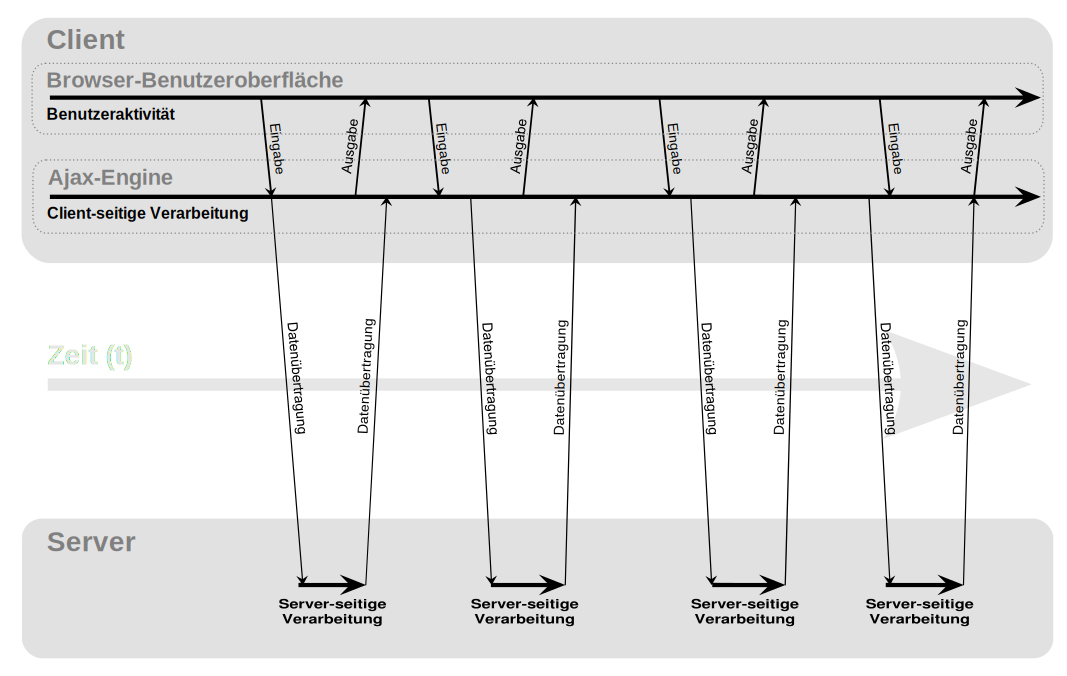
\includegraphics[width=\linewidth]{images/diagram-ajax}
  \caption{Ajax Modell einer Web-Anwendung (asynchrone Datenübertragung)}
  \captionsetup{font={footnotesize,bf,it}}
  \caption*{Quelle: Wikipedia}
  \label{fig:diagram-ajax}
\end{figure}

\subsubsection{WebSockets}

Websockets sind ein in HTML5 neu eingeführter Standard zur bidirektionalen  Kommunikation zwischen
Browser und Webserver. Hierbei wird anders als bei  AJAX eine direkte TCP-Verbindung hergestellt.
Diese Verbindung kann sowohl von  Browser-, als auch von Serverseite aus gleichartig verwendet
werden. Das macht es  unnötig, wie bei AJAX wiederholte Anfragen oder Anfragen ohne Zeitbegrenzung
zu  stellen, um Informationen vom Server zu erhalten, wenn diese verfügbar werden. Ein weiterer
Vorteil gegenüber HTTP-Anfragen ist, dass durch die direkte permanente Verbindung kein
Nachrichtenkopf mehr nötig ist. Das macht es deutlich  effizienter, viele kleine Nachrichten zu
versenden.

Zum Aufbau einer WebSocket Verbindung wird einmalig zu Beginn eine \acr{http} Anfrage vom Browser
gestellt, die der Server dann im Erfolgsfall mit der Eröffnung des WebSockets beantwortet.
\cite{websockets}

\clearpage

\subsection{JavaScript-Bibliotheken}

Über den HTML5 Standard hinaus werden für die Strukturierung der Anwendung einige
\acr{js}-Bibliotheken benötigt, die im Folgenden kurz erläutert werden.

\subsubsection{jQuery}

Die Bibliothek \textit{jQuery}\footnote{http://www.jquery.com} ist heute ein defacto-Standard in der
Webentwicklung. In erster Linie erleichtert es den Zugriff und die Manipulation des \acr{dom},
bietet aber darüber hinaus zahlreiche Vereinfachungen im Umgang mit alltäglichen Aufgaben der
Webentwickling. Besonders erwähnenswert ist hierbei auch die \acr{ajax}-Abstraktion. Eine gute
Einführung in jQuery bietet \cite{jquery}.

\subsubsection{Backbone und Underscore}

\textit{Backbone}\footnote{backbonejs.org} ist eine Bibliothek, die der Strukturierung von
sogenannten \textit{single-page}-\acr{js}-Anwendungen dient. Backbone baut auf der allgemeinen
\textit{Underscore}\footnote{underscorejs.org}-Bibliothek auf, die einige Erleicherungen im Umgang
mit Daten in \acr{js} bietet.. Backbone führt das Model-View-Controller Konzept in
Browseranwendungen ein und bietet hierfür einige Prototypen, von denen abgeleitet werden kann um
eigene Modelle und Views zu implementieren, die dann über Events deklarativ miteinander verküpft
werden können.

Besonders interessant ist die Möglichkeit, die im \acr{html}5 Standard neu eingeführte
\textit{History API} in Backbone zur Navigation zu verwenden. Dadurch ist es möglich in einer
\acr{js}-Anwendung, welche die Seite nicht neu aufbaut, sondern immer nur Teile verändert,
Navigation einzuführen, sodass der Benutzer zwischen den Zuständen Navigieren kann. Hierfür bietet
Backbone die sogenannten \texttt{Router} in denen von URLs auf Zustände der Anwendung und umgekehrt
abgebildet werden kann. Eine gute Einführung in die Bibliothek findet sich in \cite{backbone}.

\subsubsection{RequireJS}
\label{sec:requirejs}

Da JavaScript von Haus aus keine Möglichkeit der Modularisierung bietet, komplexe Anwendungen
jedoch ohne Modularisierung kaum wartbar bleiben, haben sich unterschiedliche Lösungsansätze für
dieses Problem entwickelt. Einer der  umfassendsten ist die Bibliothek \textit{RequireJS}.

Mit der Funktion \texttt{define} können Module in Form von Funktionsdefinitionen  definiert werden.
Alle lokalen Variablen in dem Modul sind anders als bei  normalen Scripten außerhalb nicht mehr
sichtbar, da sie innerhalb einer  Funktion definiert wurden. Das Funktionsergebnis ist das was nach
außen sichtbar  ist. Dies kann ein beliebiges Objekt (also auch eine Funktion) sein.

Die so definierten Module können Abhängigkeiten untereinander spezifizieren,  indem der
\texttt{define}-Funktion eine Liste von Modulen übergeben wird, die  das aktuelle Modul benötigt.
Die \textit{RequireJS}-Bibliothek sorgt dann dafür,  dass diese Module geladen werden bevor das
aktuelle Modul ausgeführt wird.

RequireJS erlaubt es, den  \acr{js}-Code für den Produktiveinsatz zu optimieren. Dafür
gibt es  das sogenannte \textit{r.js}-Script, das unter anderm alle Abhängigkeiten in eine Datei
zusammenfasst und den Code durch entfernen von Whitespaces und Kommentaren  sowie umbenennen
von Variablennamen verkürzt. Zur Entwicklungszeit ist dieser nicht mehr lesbare Code nicht
erwünscht. Deswegen bietet das Play Framework (Siehe Abschnitt \ref{sec:play}) eine integrierte
Version von RequireJS, die automatisch den lesbaren Code zur Entwicklungszeit  bereitstellt, im
Produktiveisatz jedoch den optimierten.